% !TeX program = xelatex
% !TeX encoding = UTF-8
% !TeX root    = document_template.tex
\documentclass{../mirea-prog-lang}

\usepackage{hyperref}

\usepackage{graphicx}
\usepackage{pdfpages}
\usepackage{titlesec}
\usepackage{float}

\titlespacing*{\section}{0pt}{0pt}{0pt}
\titlespacing*{\subsection}{0pt}{0pt}{0pt}
\titlespacing*{\subsubsection}{0pt}{0pt}{0pt}

\setlength{\cftbeforesecskip}{0pt} % Addtional space between sections in toc
\setlength{\cftsecindent}{0pt} % Remove indent in toc for \section
\setlength{\cftsubsecindent}{0pt} % Remove indent in toc for \subsection
\setlength{\cftsubsubsecindent}{0pt} % Remove indent in toc for \subsubsection

\begin{document}

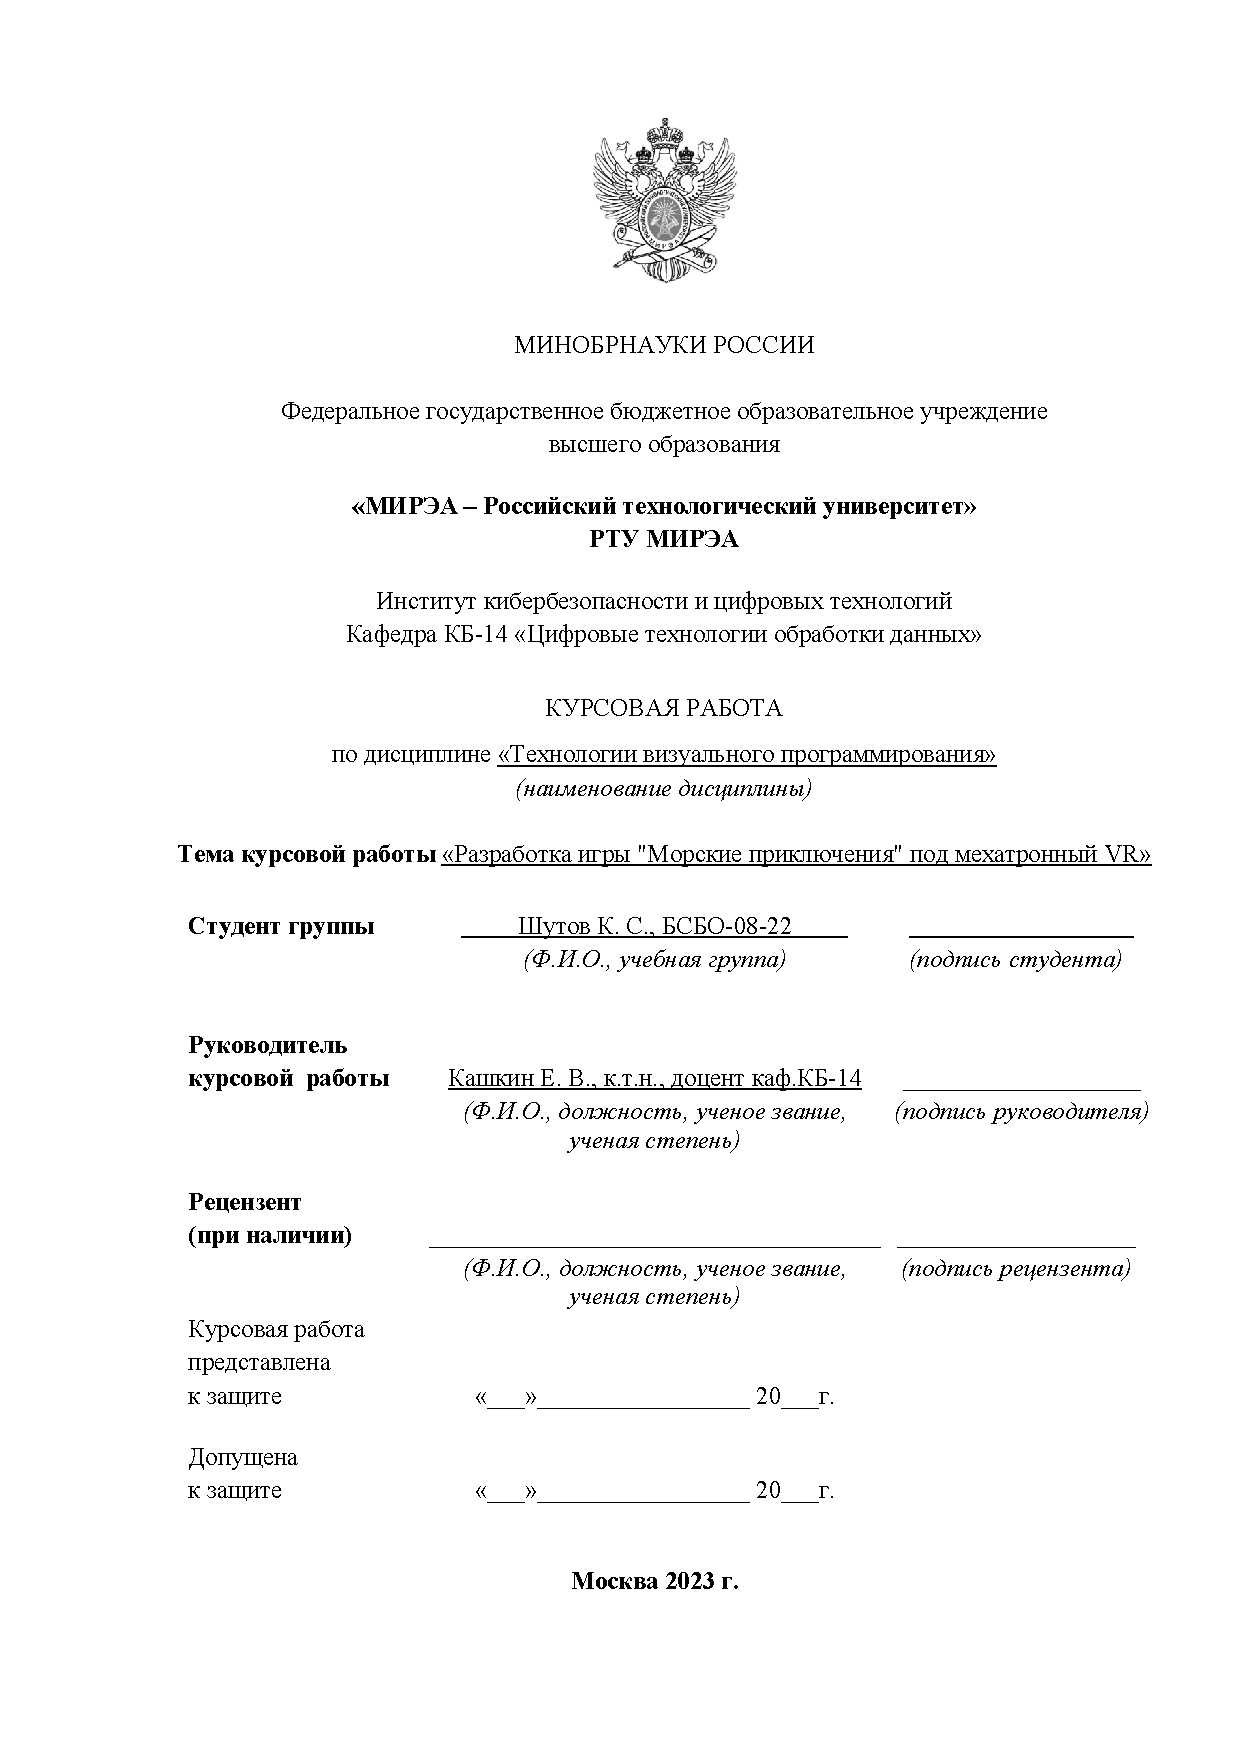
\includepdf[pages=-]{../../TitlePage.pdf}	

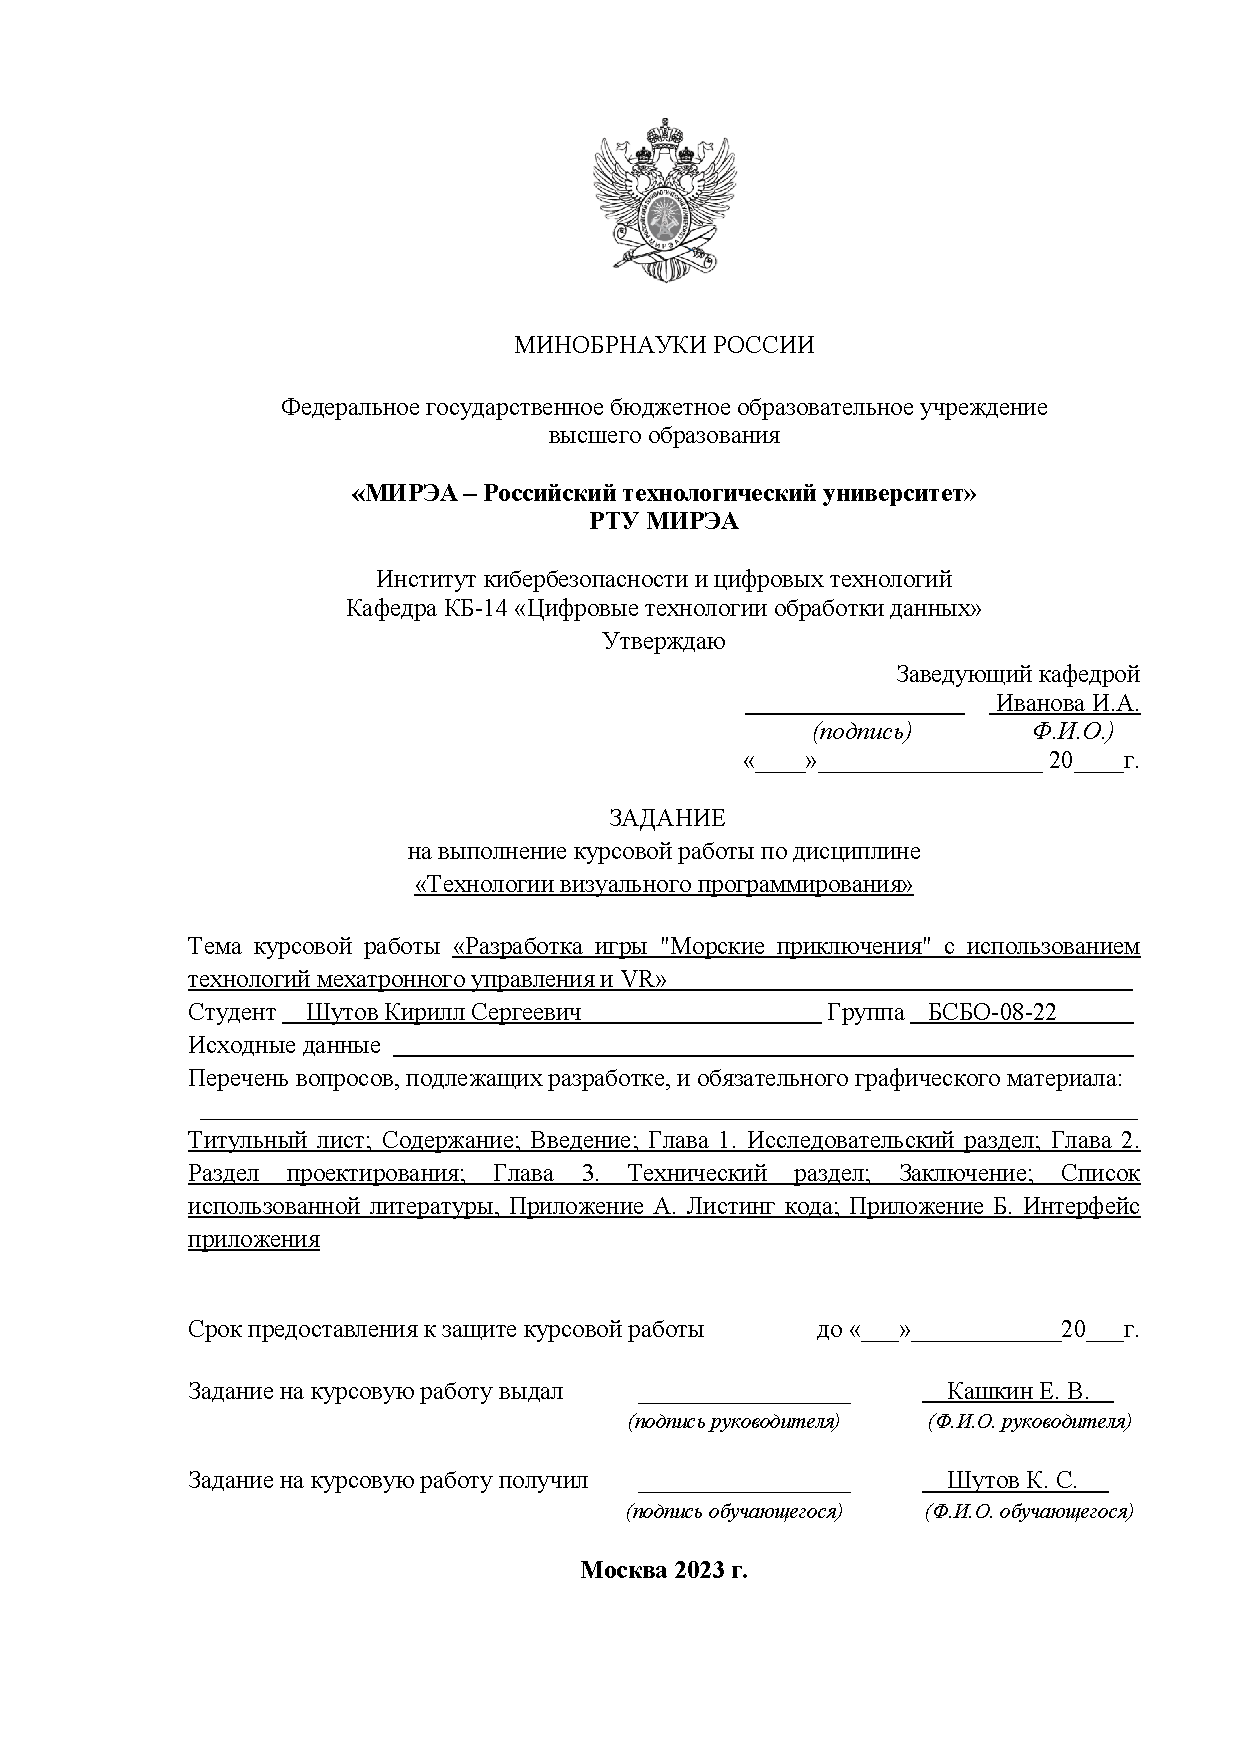
\includepdf[pages=-]{../../TaskPage.pdf}	

\tableofcontents

\section*{Введение}
\phantomsection
\addcontentsline{toc}{section}{Введение}

Игры являются актуальным и популярным видом время провождения в современном мире. Они стали неотъемлемой частью культуры и развлечения доступной на различных устройствах. Более того, развитие технологий позволяет создавать все более захватывающие и реалистичные игровые миры. В настоящее время помимо привычных нам устройст для запуска игр таких как компьютер, телефон, игровая консоль есть и другие, позволяющие расширить доступные игровые возможности, такие как технологии мехатронного управления и виртуальная реальность.

Целью данной курсовой работе является разработка игры "Морские приключения" с использованием технологий мехатронного управления и VR.

Игрок будет играть за персонажа, управляющего подводной лодкой, которому нужно догонять морских существ обитающих в аквариуме.

\begin{itemize}
	\item[] Во время разработки планируется провести:
	\item проектирование концепции игры;
	\item подбор ассетов для конечного продукта;
	\item моделирование игрового пространства;
	\item разработка основных игровых механик;
	\item замена грейбокс моделей на подобранные ассеты;
	\item прототипирование искусственного интеллекта морсих существ и настройка их анимации;
	\item продумывание мотивации для игрока;
	\item тестирование и отладка игры.
\end{itemize}

Особое внимание будет уделено виртуальной реальности, что позволит погрузиться в игровой мир, предоставляя уникальный опыт, который нельзя получить в традиционных играх. Одним из главных его преимуществ является то, что игра является уникальной благодаря использованию технологии мехатронного управления.

\begin{itemize}
	\item[] Будут пройдены этапы разработки игры, такие как:
	\item изучение существующих аналогов;
	\item создание концепции игры;
	\item реализации конечного продукта.
\end{itemize}

\section{Теоретическая часть}

Для поиска идеальных решений в программном продукте следует оценить разработки аналогичных продуктов.
При поиске в различных ресурсах можно найти множество игр в про подводные погружения, но реализаций где игрок мог бы почуствовать себя под водой управляя подводной лодкой и находясь в капсуле виртуальной реальности, нет. Исследование и анализ уже существующих похожих игр поможет выявить их преимущества и недостатки, что позволит учесть их при разработке своей игры.

\subsection{Анализ существующих решений}

В этой главе будут рассмотрены несколько игр, посвященных подводным приключениям. Они будут оцениваться согласно специальным критериям, которые были тщательно подобраны, учитывая особенности данной тематики. Эти критерии наилучшим образом отразят качество и характеристики задумки:

\begin{itemize}
	\item графика и визуальный стиль. Позволят оценить качество визуальных элементов в игре, включая дизайн подводного мира, анимацию и общий визуальный стиль, который способствует погружению игрока в атмосферу подводных приключений.
	
	\item наличие виртуальной реальности. Поддерживает ли игра виртуальную реальность (VR), так как VR может существенно повысить уровень иммерсии и вовлеченности игрока.
	
	\item игровой геймплей и управление. Позволят проанализировать, насколько хорошо разработан игровой процесс, включая механики плавания, исследования подводного мира и боевые действия. Управление также будет оценено на удобство и интуитивность.
	
	\item иммерсия и атмосфера. Позволят определить, насколько успешно игры передают атмосферу подводных глубин, включая звуковое сопровождение, звуковые эффекты и общую атмосферу, способствующую погружению игрока в мир под водой.
	
	\item оценки пользователей. Мнение игроков также будет учтено в оценке. Проанализировав отзывы и оценки пользователей, чтобы узнать, как игры были приняты в игровом сообществе и насколько они соответствуют ожиданиям игроков.
\end{itemize}

После тщательного анализа каждой игры по указанным критериям, будет возможно сделать объективные выводы о качестве и привлекательности каждой из них в контексте подводных приключений.

\begin{itemize}
	\item theBlu VR - это виртуальная реальность (VR) приключение, предоставляющее игрокам возможность исследовать подводный мир океана в захватывающем 3D формате. theBlu VR погружает игроков в удивительные морские глубины, где они могут встретить разнообразные морские создания и насладиться великолепной визуализацией подводного мира. Эта VR-игра не ограничивается элементами геймплея, но больше ориентирована на создание невероятных визуальных впечатлений и обогащение знаний о подводной фауне и флоре.
	
	\item Subnautica - это приключенческая игра с элементами выживания и исследования, разработанная в открытом океане на чужой планете. Игроки оказываются в роли выжившего после крушения на этой планете и должны исследовать огромный подводный мир, собирать ресурсы, строить базы и изучать тайны атмосферы этого удивительного места. Subnautica отличается великолепной графикой и невероятной атмосферой, и она привлекла множество игроков своими увлекательными приключениями и опасностями, которые подстерегают в подводных глубинах.
	
	\item Ocean Rift - это ещё одна VR-игра, которая транспортирует игроков в подводный мир, предлагая уникальные виртуальные приключения. Игроки могут исследовать разнообразные морские сценарии, встречая разнообразных подводных обитателей, такие как акулы, дельфины и многие другие виды морской жизни. Эта игра создает непередаваемое ощущение присутствия в океане и позволяет игрокам узнать больше о морских экосистемах и их важности. Ocean Rift воплощает в себе идею виртуального обучения и развлечения, сочетая в себе образовательные и развлекательные аспекты.
\end{itemize}

\subsection{theBlu VR}

Графика и визуальный стиль:
theBlu VR впечатляет своей потрясающей визуальной графикой и детализацией подводного мира. Он является одной из самых красивых игр в мире виртуальной реальности. Модели морских существ и кораллов выглядят невероятно реалистично.

Виртуальная реальность:
Эта игра специально создана для виртуальной реальности, что делает ее полностью подходящей для VR. Вы погружаетесь в подводный мир, словно находитесь под водой.

Игровой геймплей и управление:
Игровой геймплей в theBlu VR не нацелен на бои или задачи, а скорее на исследование и наблюдение за подводными существами. Управление простое и интуитивное, что делает игру доступной для новичков.

Иммерсия и атмосфера:
Игра предоставляет невероятно глубокую иммерсию и атмосферу. Вы ощущаете себя настоящим наблюдателем под водой, и это создает удивительное ощущение присутствия.

Оценки пользователей:
theBlu VR получила положительные отзывы от пользователей, оцененные в основном на высокие баллы за визуализацию и атмосферу.

\subsection{Subnautica}

Графика и визуальный стиль:
Графика в Subnautica является красочной и подробной. Мир подводного ландшафта кажется живым и разнообразным, с огромным разнообразием подводных существ и растений.

Виртуальная реальность:
Хотя официальная версия игры Subnautica не поддерживает виртуальную реальность, существуют модификации, позволяющие играть в игру в VR.

Игровой геймплей и управление:
Subnautica предоставляет отличный игровой геймплей с элементами выживания и исследования. Управление в VR может потребовать некоторой настройки, но оно в целом удобно.

Иммерсия и атмосфера:
Игра создает потрясающую атмосферу, погружая вас в мир подводных глубин, полный опасностей и таинств. Иммерсия является одним из сильных сторон этой игры.

Оценки пользователей:
Subnautica получила высокие оценки пользователей и признание за ее увлекательный геймплей и атмосферу.

\subsection{Ocean Rift}

Графика и визуальный стиль:
Ocean Rift имеет невероятно красочную и реалистичную графику, что делает подводный мир живым и увлекательным для исследования.

Виртуальная реальность:
Эта игра также специально создана для виртуальной реальности, что позволяет вам ощутить себя настоящим подводным исследователем.

Игровой геймплей и управление:
Ocean Rift ориентирована на образование и развлечение, предлагая множество интерактивных моментов, таких как наблюдение за подводными существами и изучение морских экосистем. Управление интуитивное и легко осваивается.

Иммерсия и атмосфера:
Игра обеспечивает глубокую иммерсию и погружает вас в чудесный мир подводной жизни с его уникальной атмосферой.

Оценки пользователей:
Ocean Rift получила положительные отзывы от пользователей, особенно за ее образовательную ценность и визуальные эффекты.

\subsection{Сравнительный анализ}

Сравнительный анализ для каждой из игр, а также таблица с краткой сводкой (См. таблицу~\ref{tab:1} на~с.~\pageref{tab:1}.):

\begin{table}[H]
	\caption{Сравнительный анализ}
	\centering
	\begin{tabular}{ |p{3cm}|p{4cm}|p{4cm}|p{4cm}| }
		\hline
		{Критерий} & {theBlu VR} & {Subnautica} & {Ocean Rift}\\ \hline
		
		{Графика и визуальный стиль} & {Очень реалистичная и детализированная подводная графика с потрясающими морскими существами и кораллами.} & {Красочная и детальная графика подводного мира с разнообразием подводных существ и растений.} & {Красочная и реалистичная графика подводной среды с уникальными видами подводной жизни.} \\ \hline
	\end{tabular}
	\label{tab:1}
\end{table}

\begin{table}[H]
	\begin{tabular}{ |p{2.75cm}|p{4.2cm}|p{4.2cm}|p{4.2cm}| }
		\hline
		{Виртуальная реальность} & {Да} & {Модификации доступны} & {Да} \\ \hline
		
		{Игровой геймплей и управление} & {Исследование и наблюдение без акцента на боях. Простое и интуитивное управление.} & {Выживание и исследование с удовлетворительным управлением. Можно потребоваться настройка для VR.} & {Исследование и образовательные моменты, интуитивное управление.} \\ \hline
		
		{Иммерсия и атмосфера} & {Потрясающая иммерсия и ощущение присутствия под водой.} & {Глубокая атмосфера с увлекательными таинствами подводного мира.} & {Увлекательная атмосфера с акцентом на образование.} \\ \hline
		
		{Оценки пользователей} & {Положительные отзывы с высокими оценками за визуализацию и атмосферу.} & {Высокие оценки за увлекательный геймплей и атмосферу.} & {Положительные отзывы с признанием образовательной ценности и визуальных эффектов.} \\ \hline
	\end{tabular}
\end{table}

theBlu VR предоставляет потрясающую визуальную графику и полную иммерсию, но ограничивает игровой процесс более формальным наблюдением и отсутствием игровых задач.

Subnautica предлагает красочный мир подводного исследования и выживания, с потрясающей атмосферой. Несмотря на то, что официальная версия не поддерживает VR, существуют модификации для игры в виртуальной реальности.

Ocean Rift фокусируется на образовании и исследовании мира подводной жизни, предоставляя уникальные образовательные моменты и красочную графику.

\subsection{Выбор инструментария и технологий}

При разработке игры могут понадобится следующие инструменты и технологии:

\begin{itemize}
	\item игровые движки для создания и редактирования игровых уровней и сцен, например Unity, Unreal Engine, GameMaker Studio, Construct, Godot;
	\item языки программирования, такие как C\#, C++, JavaScript, Python, Lua, для написания игровых скриптов, плагинов и расширений;
	\item редакторы кода и интегрированные среды разработки (IDE) для написания и отладки игрового кода, например Visual Studio, JetBrains Rider, Eclipse;
	\item системы контроля версий для хранения и управления исходным кодом, например Git, SVN, Mercurial;
	\item устройства для виртуальной реальности, например Oculus Rift, HTC Vive, PlayStation VR, Google Daydream, Samsung Gear VR.
\end{itemize}

Для реализации проекта будет использован следующий инструментальный аппарат и технологии:

\begin{itemize}
	\item Unity - выбран в качестве игрового движка, так как он предоставляет мощные инструменты для разработки трехмерных игр, имеет большое сообщество разработчиков в отличии от других игровых движков, богатую документацию, широкие возможности для создания игровой логики и взаимодействия объектов, а также имеет множество готовых решений и плагинов;
	\item язык программирования C\# - выбран, потому что он широко используется для разработки игр на платформе Unity, имеет хорошую производительность, мощную библиотеку .NET Framework и имеет удобный синтаксис;
	\item интегрированная среда разработки (IDE) JetBrains Rider выбрана как основное средство разработки, так как она обладает широким набором функций для написания, отладки и тестирования кода на C\#, интеграцией с популярными системами контроля версий и возможностью подключения к Unity;
	\item Git - выбран в качестве системы контроля версий, так как он позволяет эффективно управлять изменениями в исходном коде, создавать ветки для экспериментов и легко возвращаться к предыдущим версиям;
	\item Oculus Rift был выбран как устройство виртуальной реальности, которое обеспечивает отличный уровень управления, что позволит игрокам полностью погрузиться в игровой мир. Он также имеет хорошую поддержку и инструменты разработки для VR-игр.
\end{itemize}

Также, выбор инструментария был основан на их профессиональной репутации, способности интеграции между собой. Кроме того, Unity является одним из наиболее популярных игровых движков, который имеет широкое сообщество разработчиков и обеспечивает множество готовых решений для различных аспектов игровой разработки.

\subsection{Постановка задачи}

Будет разработана VR игра, которая позволит пользователям погрузиться в виртуальный мир и взаимодействовать с объектами. Главной задачей будет создание качественного игрового контента и реализация интуитивно понятного интерфейса управления для наиболее удобного и естественного взаимодействия игрока с игровым миром.

Для достижения данной задачи должны быть выполнены следующие шаги:

\begin{itemize}
	\item изучение технологий виртуальной реальности и их применение в игровой разработке;
	\item исследование различных реферансов и определение их основных характеристик и механик, а также выявление элементов, которые можно перенести в VR-окружение;
	\item составление дизайна с описанием игровых механик и геймплея;
	\item подбор ассетов которые будут использованы в игре;
	\item моделирование игрового пространство в Unity, включая уровни и сцены, и настройка игровых объектов;
	\item разработка игровых механик;
	\item замена грейбокс моделей на модели объектов и настройка их коллизий;
	\item реализовать аудио эффекты и музыкальное сопровождение игры;
	\item оптимизировать игру для работы в виртуальной реальности;
	\item исправить ошибки и улучшить игру на основе результатов тестирования;
	\item документировать разработку игры и написать отчет о выполненной работе.
\end{itemize}

Общая задача состоит в том, чтобы создать уникальную и увлекательную игру в виртуальной реальности про подводные приключения, которая обеспечивает высокую переиграбельность, интересный геймплей и визуальные эффекты.

\subsection{Вывод}

В первой главе было проанализировано несколько существующих решений в области игр про подводные приключения, выявлены их преимущества и недостатки. Проанализированы различные подходы к созданию. На основе проведенного анализа были определены принципы, которые поставлены во главе процесса разработки игры.

Был выбран подходящий инструментарий и технологии, которые позволят реализовать задачи проекта наиболее эффективным способом.
Поставлена задача на разработку игры, она разделена на пункты для более удобной разработки, это будет основной целью всей работы.

Исходя из проведенного исследования, разработка VR-игры является актуальной задачей в настоящее время. Данная тематика имеет свою аудиторию и пользуется популярностью среди геймеров.

Выбранный инструментарий и технологии позволяют реализовать все задачи проекта и достичь поставленных целей.

\section{Практическая часть}

Моя практическая часть.

\section*{Заключение}
\phantomsection
\addcontentsline{toc}{section}{Заключение}

Моё заключение.

\begin{thebibliography}{99\kern\bibindent}
	\bibitem{bib:mybook} Моя книга.
	\bibitem{bib:mybook2} Моя вторая книга. 
\end{thebibliography}

\appendix

\section{Моё приложение}

Моё приложение.

\section{Моё второе приложение}

Моё второе приложение.

\end{document}